% Generated by Sphinx.
\def\sphinxdocclass{report}
\documentclass[a4paper,10pt,english]{sphinxmanual}
\usepackage[utf8]{inputenc}
\DeclareUnicodeCharacter{00A0}{\nobreakspace}
\usepackage[T1]{fontenc}
\usepackage{babel}
\usepackage{times}
\usepackage[Bjarne]{fncychap}
\usepackage{longtable}
\usepackage{sphinx}
\usepackage{multirow}


\title{PropGen Documentation}
\date{February 19, 2012}
\release{0}
\author{Holger Karl}
\newcommand{\sphinxlogo}{}
\renewcommand{\releasename}{Release}
\makeindex

\makeatletter
\def\PYG@reset{\let\PYG@it=\relax \let\PYG@bf=\relax%
    \let\PYG@ul=\relax \let\PYG@tc=\relax%
    \let\PYG@bc=\relax \let\PYG@ff=\relax}
\def\PYG@tok#1{\csname PYG@tok@#1\endcsname}
\def\PYG@toks#1+{\ifx\relax#1\empty\else%
    \PYG@tok{#1}\expandafter\PYG@toks\fi}
\def\PYG@do#1{\PYG@bc{\PYG@tc{\PYG@ul{%
    \PYG@it{\PYG@bf{\PYG@ff{#1}}}}}}}
\def\PYG#1#2{\PYG@reset\PYG@toks#1+\relax+\PYG@do{#2}}

\def\PYG@tok@gd{\def\PYG@tc##1{\textcolor[rgb]{0.63,0.00,0.00}{##1}}}
\def\PYG@tok@gu{\let\PYG@bf=\textbf\def\PYG@tc##1{\textcolor[rgb]{0.50,0.00,0.50}{##1}}}
\def\PYG@tok@gt{\def\PYG@tc##1{\textcolor[rgb]{0.00,0.25,0.82}{##1}}}
\def\PYG@tok@gs{\let\PYG@bf=\textbf}
\def\PYG@tok@gr{\def\PYG@tc##1{\textcolor[rgb]{1.00,0.00,0.00}{##1}}}
\def\PYG@tok@cm{\let\PYG@it=\textit\def\PYG@tc##1{\textcolor[rgb]{0.25,0.50,0.56}{##1}}}
\def\PYG@tok@vg{\def\PYG@tc##1{\textcolor[rgb]{0.73,0.38,0.84}{##1}}}
\def\PYG@tok@m{\def\PYG@tc##1{\textcolor[rgb]{0.13,0.50,0.31}{##1}}}
\def\PYG@tok@mh{\def\PYG@tc##1{\textcolor[rgb]{0.13,0.50,0.31}{##1}}}
\def\PYG@tok@cs{\def\PYG@tc##1{\textcolor[rgb]{0.25,0.50,0.56}{##1}}\def\PYG@bc##1{\colorbox[rgb]{1.00,0.94,0.94}{##1}}}
\def\PYG@tok@ge{\let\PYG@it=\textit}
\def\PYG@tok@vc{\def\PYG@tc##1{\textcolor[rgb]{0.73,0.38,0.84}{##1}}}
\def\PYG@tok@il{\def\PYG@tc##1{\textcolor[rgb]{0.13,0.50,0.31}{##1}}}
\def\PYG@tok@go{\def\PYG@tc##1{\textcolor[rgb]{0.19,0.19,0.19}{##1}}}
\def\PYG@tok@cp{\def\PYG@tc##1{\textcolor[rgb]{0.00,0.44,0.13}{##1}}}
\def\PYG@tok@gi{\def\PYG@tc##1{\textcolor[rgb]{0.00,0.63,0.00}{##1}}}
\def\PYG@tok@gh{\let\PYG@bf=\textbf\def\PYG@tc##1{\textcolor[rgb]{0.00,0.00,0.50}{##1}}}
\def\PYG@tok@ni{\let\PYG@bf=\textbf\def\PYG@tc##1{\textcolor[rgb]{0.84,0.33,0.22}{##1}}}
\def\PYG@tok@nl{\let\PYG@bf=\textbf\def\PYG@tc##1{\textcolor[rgb]{0.00,0.13,0.44}{##1}}}
\def\PYG@tok@nn{\let\PYG@bf=\textbf\def\PYG@tc##1{\textcolor[rgb]{0.05,0.52,0.71}{##1}}}
\def\PYG@tok@no{\def\PYG@tc##1{\textcolor[rgb]{0.38,0.68,0.84}{##1}}}
\def\PYG@tok@na{\def\PYG@tc##1{\textcolor[rgb]{0.25,0.44,0.63}{##1}}}
\def\PYG@tok@nb{\def\PYG@tc##1{\textcolor[rgb]{0.00,0.44,0.13}{##1}}}
\def\PYG@tok@nc{\let\PYG@bf=\textbf\def\PYG@tc##1{\textcolor[rgb]{0.05,0.52,0.71}{##1}}}
\def\PYG@tok@nd{\let\PYG@bf=\textbf\def\PYG@tc##1{\textcolor[rgb]{0.33,0.33,0.33}{##1}}}
\def\PYG@tok@ne{\def\PYG@tc##1{\textcolor[rgb]{0.00,0.44,0.13}{##1}}}
\def\PYG@tok@nf{\def\PYG@tc##1{\textcolor[rgb]{0.02,0.16,0.49}{##1}}}
\def\PYG@tok@si{\let\PYG@it=\textit\def\PYG@tc##1{\textcolor[rgb]{0.44,0.63,0.82}{##1}}}
\def\PYG@tok@s2{\def\PYG@tc##1{\textcolor[rgb]{0.25,0.44,0.63}{##1}}}
\def\PYG@tok@vi{\def\PYG@tc##1{\textcolor[rgb]{0.73,0.38,0.84}{##1}}}
\def\PYG@tok@nt{\let\PYG@bf=\textbf\def\PYG@tc##1{\textcolor[rgb]{0.02,0.16,0.45}{##1}}}
\def\PYG@tok@nv{\def\PYG@tc##1{\textcolor[rgb]{0.73,0.38,0.84}{##1}}}
\def\PYG@tok@s1{\def\PYG@tc##1{\textcolor[rgb]{0.25,0.44,0.63}{##1}}}
\def\PYG@tok@gp{\let\PYG@bf=\textbf\def\PYG@tc##1{\textcolor[rgb]{0.78,0.36,0.04}{##1}}}
\def\PYG@tok@sh{\def\PYG@tc##1{\textcolor[rgb]{0.25,0.44,0.63}{##1}}}
\def\PYG@tok@ow{\let\PYG@bf=\textbf\def\PYG@tc##1{\textcolor[rgb]{0.00,0.44,0.13}{##1}}}
\def\PYG@tok@sx{\def\PYG@tc##1{\textcolor[rgb]{0.78,0.36,0.04}{##1}}}
\def\PYG@tok@bp{\def\PYG@tc##1{\textcolor[rgb]{0.00,0.44,0.13}{##1}}}
\def\PYG@tok@c1{\let\PYG@it=\textit\def\PYG@tc##1{\textcolor[rgb]{0.25,0.50,0.56}{##1}}}
\def\PYG@tok@kc{\let\PYG@bf=\textbf\def\PYG@tc##1{\textcolor[rgb]{0.00,0.44,0.13}{##1}}}
\def\PYG@tok@c{\let\PYG@it=\textit\def\PYG@tc##1{\textcolor[rgb]{0.25,0.50,0.56}{##1}}}
\def\PYG@tok@mf{\def\PYG@tc##1{\textcolor[rgb]{0.13,0.50,0.31}{##1}}}
\def\PYG@tok@err{\def\PYG@bc##1{\fcolorbox[rgb]{1.00,0.00,0.00}{1,1,1}{##1}}}
\def\PYG@tok@kd{\let\PYG@bf=\textbf\def\PYG@tc##1{\textcolor[rgb]{0.00,0.44,0.13}{##1}}}
\def\PYG@tok@ss{\def\PYG@tc##1{\textcolor[rgb]{0.32,0.47,0.09}{##1}}}
\def\PYG@tok@sr{\def\PYG@tc##1{\textcolor[rgb]{0.14,0.33,0.53}{##1}}}
\def\PYG@tok@mo{\def\PYG@tc##1{\textcolor[rgb]{0.13,0.50,0.31}{##1}}}
\def\PYG@tok@mi{\def\PYG@tc##1{\textcolor[rgb]{0.13,0.50,0.31}{##1}}}
\def\PYG@tok@kn{\let\PYG@bf=\textbf\def\PYG@tc##1{\textcolor[rgb]{0.00,0.44,0.13}{##1}}}
\def\PYG@tok@o{\def\PYG@tc##1{\textcolor[rgb]{0.40,0.40,0.40}{##1}}}
\def\PYG@tok@kr{\let\PYG@bf=\textbf\def\PYG@tc##1{\textcolor[rgb]{0.00,0.44,0.13}{##1}}}
\def\PYG@tok@s{\def\PYG@tc##1{\textcolor[rgb]{0.25,0.44,0.63}{##1}}}
\def\PYG@tok@kp{\def\PYG@tc##1{\textcolor[rgb]{0.00,0.44,0.13}{##1}}}
\def\PYG@tok@w{\def\PYG@tc##1{\textcolor[rgb]{0.73,0.73,0.73}{##1}}}
\def\PYG@tok@kt{\def\PYG@tc##1{\textcolor[rgb]{0.56,0.13,0.00}{##1}}}
\def\PYG@tok@sc{\def\PYG@tc##1{\textcolor[rgb]{0.25,0.44,0.63}{##1}}}
\def\PYG@tok@sb{\def\PYG@tc##1{\textcolor[rgb]{0.25,0.44,0.63}{##1}}}
\def\PYG@tok@k{\let\PYG@bf=\textbf\def\PYG@tc##1{\textcolor[rgb]{0.00,0.44,0.13}{##1}}}
\def\PYG@tok@se{\let\PYG@bf=\textbf\def\PYG@tc##1{\textcolor[rgb]{0.25,0.44,0.63}{##1}}}
\def\PYG@tok@sd{\let\PYG@it=\textit\def\PYG@tc##1{\textcolor[rgb]{0.25,0.44,0.63}{##1}}}

\def\PYGZbs{\char`\\}
\def\PYGZus{\char`\_}
\def\PYGZob{\char`\{}
\def\PYGZcb{\char`\}}
\def\PYGZca{\char`\^}
\def\PYGZsh{\char`\#}
\def\PYGZpc{\char`\%}
\def\PYGZdl{\char`\$}
\def\PYGZti{\char`\~}
% for compatibility with earlier versions
\def\PYGZat{@}
\def\PYGZlb{[}
\def\PYGZrb{]}
\makeatother

\begin{document}

\maketitle
\tableofcontents
\phantomsection\label{index::doc}


Contents:


\chapter{Why this tool?}
\label{motivation::doc}\label{motivation:welcome-to-propgen-s-documentation}\label{motivation:why-this-tool}
Writing an application for a research project is a challenging task: good ideas are needed, background research checks, a research hypothesis and a research program have to be formulated. When applying for a larger project, this is typically done by a group of people, coming from different organizations. A lot of work goes into the creative process - the mere act of writing the proposal, collecting information about the program structure, putting it in Gantt charts and tables of deliverables etc. should get out of the way!

Anybody who has tried to write a proposal for one of the European Union's Framework Programs knows that it can be a cumbersome process. The EU provides a relatively strict template which information to provide: information about work packages, tasks, deliverables, milestones, Gantt charts, etc. Much of this information is repeated at several places in the document, in various forms of presentation (tables, charts, free text). Merely keeping this information in synch can be a formidable challenge, in particular, when several people work on a proposal. To make matters worse, the EU only provides an MS Word template (and not a particularly well done one, either). There is no support to get all the administrative work out of the way.

This was the very situation we were in when we developed a proposal for a reasonably large EU proposal (an integrated project with about 15 partners). Instead of going down the Word-road, we decided to put all the information on a Wiki and to generate the actual proposal from there, using LaTeX to typeset the actual document and generating all the administrative information automatically. This has three main advantages:
\begin{itemize}
\item {} 
Wikis are easy to use even for novel users who are not used to using version control systems for collaborative work (let alone trying to distribute these files via email). Wikis naturally split up text in separate sections, circumventing the often problematic features of word processors to split up a document in smaller files.

\item {} 
All the administrative information only needs to be entered ONCE. All possible presentations are automatically generated. They are guaranteed to stay synchronized. There is no time wasted for such work. Even non-trivial operations can be done until late in the proposal preparation without any risk (e.g., we decided to move a deliverable around a few hours before proposal submission - that would have been impossible with conventional tools).

\item {} 
Wikis allow us to concentrate on the content, on our research ideas. We do not have to waste time fighting with a word processor.

\end{itemize}

To give one example: a task description for a workpackage looks as described in the figure in a moinmoin wiki. This then gets translated automatically into a Gantt chart for the workpackage (and into a Gantt chart for the project as a whole, and in tables, and in ...).
\begin{figure}[htbp]
\centering
\capstart

\scalebox{0.500000}{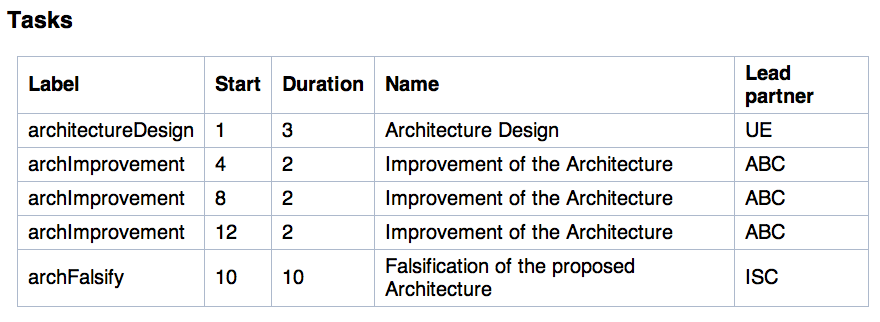
\includegraphics{wikiTasks.png}}
\caption{Example of a Wiki page, specifying several tasks for a workpackage (the architecture improvement task even has three phases).}\end{figure}
\begin{figure}[htbp]
\centering
\capstart

\scalebox{0.500000}{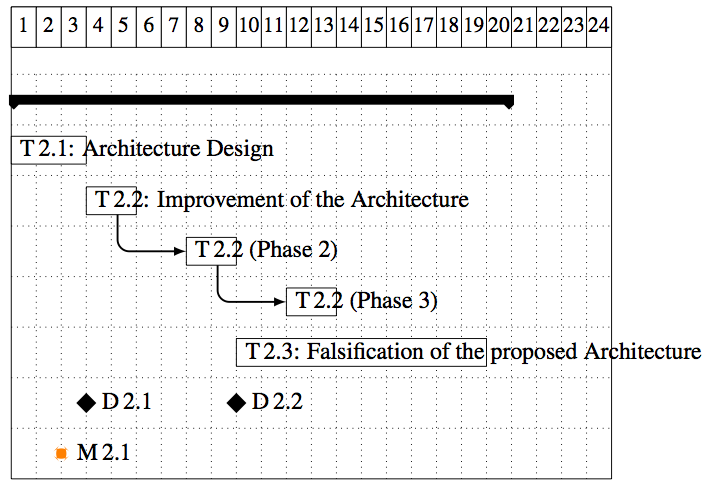
\includegraphics{WPgantt.png}}
\caption{Resulting Gantt chart from the example task table (deliverable and milestones shown in this Gantt chart are defined in other Wiki tables)}\end{figure}

Hence, the approach to go from a wiki to latex to PDF, and to submit this PDF file, has worked out nicely. It has produced a workflow that was reasonably easy for everybody, with full version control support without less IT-savy users needing to worry about it.

We felt that such a tool might be beneficial for a wider audience. So here it is - feel free to use it, to modify it, and to write interesting proposals using it. Our hope is that it will free up time from the mundane and boring tasks and enable all of us to concentrate more on the creative aspects of research.

\emph{Holger Karl}

PS: When I write ``we'', I refer to the team of colleagues engaged in the writing of said initial integrated research proposal. In particular, Bengt Ahlgren, Dirk Kutscher and Börje Ohlman deserve my thanks and gratitude for bearing through the rough-shot development of the inital version of this tool. I am indebted to them for constructive criticisms, ideas, and encouragement.


\chapter{Installation}
\label{installation:installation}\label{installation::doc}
How to install. Explain server vs. client installation. How to integrate with SVN.


\chapter{How to use PropGen}
\label{usage:how-to-use-propgen}\label{usage::doc}
What to put on Wiki. How to trigger builds. What should go in which tables. What to watch out for when editing.


\chapter{How to customize PropGren}
\label{customize:how-to-customize-propgren}\label{customize::doc}
How to customize the project.


\section{Simple customization}
\label{customize:simple-customization}
Turn on, off certain parts, set colors.


\section{Customize LaTeX templates}
\label{customize:customize-latex-templates}
All the stuff that happens in template/latexTemplate.cfg


\section{Complex customization}
\label{customize:complex-customization}
When you really have to work with the pyton code...


\chapter{Open Issues}
\label{openissues::doc}\label{openissues:open-issues}

\section{Known bugs}
\label{openissues:known-bugs}
None, of course :-). If you find any, let me know!


\section{Things still to do (TODO)}
\label{openissues:things-still-to-do-todo}\begin{enumerate}
\item {} 
Put the bibtex file onto the Wiki as
well. Probably better than to rely on version
control to distribute it.

\end{enumerate}


\section{Debatable aspects}
\label{openissues:debatable-aspects}\begin{enumerate}
\item {} 
The settings files could be put on the Wiki as
well. Two-edged sword: Might make it easier for
everybody to configure things, but that is a
serious downside as well. Technically, this would
not be difficult to do. Not made up my mind yet.

\end{enumerate}


\section{Ideas for future features}
\label{openissues:ideas-for-future-features}\begin{enumerate}
\item {} 
Integrate a version control system like SVN for
the produced LaTeX files

\item {} 
Generate PDF files directly from the Wiki, make
it possible to trigger that at least.

\item {} 
Integrate Etherpad into Wiki

\item {} 
Build a bridge to the financial planning of a
project.

\end{enumerate}
\begin{itemize}
\item {} 
Either by parsing from/ writing to an Excel
(or similar) spreadsheet. Relatively easy, but
hard to make this general

\item {} 
Or by putting spreadsheet-functionality onto
the wiki. Hard to do for different wiki types
(a nightmare, probably).

\end{itemize}
\begin{enumerate}
\setcounter{enumi}{4}
\item {} 
Build support for latexdiff. Possibly triggered
from wiki as well?

\item {} 
Better support for figures in both wiki in latex. One idea might be
to upload a PDF to the wiki and have the Wiki convert it to a PNG
file. And the pull the PDF file directly from the wiki, without
need to manually put it in the LaTeX figure directory.

\end{enumerate}


\chapter{Source code documentation}
\label{sourcecodedoc::doc}\label{sourcecodedoc:source-code-documentation}
The code described here lists in the bin directory. Some general remarks:
\begin{itemize}
\item {} 
The invocation sequence is pullproject -\textgreater{} generateXML -\textgreater{} latexFromWiki -\textgreater{} latexFromXML -\textgreater{} ensureSymbolicLinks

\item {} 
Details are in the makefile in the main directory

\item {} 
Many functions get passed a parameter ``config''. This is the content of settings.cfg, as parsed by the standard python configuration file parser ConfigParser.SafeConfigParser (see python library documentation for details).

\end{itemize}


\section{pullproject}
\label{sourcecodedoc:module-pullProject}\label{sourcecodedoc:pullproject}\index{pullProject (module)}
Pull the raw wiki files from wherever is specified in
settings.cfg. Store the raw wiki syntax in the wikipath directory.
\index{ensureDirectories() (in module pullProject)}

\begin{fulllineitems}
\phantomsection\label{sourcecodedoc:pullProject.ensureDirectories}\pysiglinewithargsret{\code{pullProject.}\bfcode{ensureDirectories}}{\emph{config}}{}
A small helper function that makes sure that all the
directories that are mentioned in settings.cfg PathNames section
actually exist. This can be useful after a make clean or in case
directories have been manually and inadvertently removed.

\end{fulllineitems}

\index{getPartners() (in module pullProject)}

\begin{fulllineitems}
\phantomsection\label{sourcecodedoc:pullProject.getPartners}\pysiglinewithargsret{\code{pullProject.}\bfcode{getPartners}}{\emph{masterPage}, \emph{pullInstance}, \emph{config}, \emph{parser}, \emph{verbose=False}}{}
get all the partner description files

\end{fulllineitems}

\index{getProposalStructure() (in module pullProject)}

\begin{fulllineitems}
\phantomsection\label{sourcecodedoc:pullProject.getProposalStructure}\pysiglinewithargsret{\code{pullProject.}\bfcode{getProposalStructure}}{\emph{masterPage}, \emph{pullInstance}, \emph{config}, \emph{parser}, \emph{verbose=False}}{}
Extract all the relevant files for the actual proposal text from the wiki.

\end{fulllineitems}

\index{getWorkpackages() (in module pullProject)}

\begin{fulllineitems}
\phantomsection\label{sourcecodedoc:pullProject.getWorkpackages}\pysiglinewithargsret{\code{pullProject.}\bfcode{getWorkpackages}}{\emph{masterPage}, \emph{pullInstance}, \emph{config}, \emph{parser}, \emph{verbose=False}}{}
Identify all the workpackages and download them

\end{fulllineitems}



\section{wikiParser}
\label{sourcecodedoc:wikiparser}

\subsection{The wikiParser module as such}
\label{sourcecodedoc:the-wikiparser-module-as-such}\label{sourcecodedoc:module-wikiParser}\index{wikiParser (module)}
We need to parse various wiki formats into useable latex. This module
provides an abstract base class wikiParser that implements a lot of
basic functions e.g.,  to extract tables, lists, etc.

This base class has to be subclassed to specialize for specific Wiki
syntax variants. The subclasses can be fairly slim and mostly specify
regular expressions to use (e.g., how to recognize headings).

A factory function is called to obtain an instance of such a parser.
\index{wikiParserFactory() (in module wikiParser)}

\begin{fulllineitems}
\phantomsection\label{sourcecodedoc:wikiParser.wikiParserFactory}\pysiglinewithargsret{\code{wikiParser.}\bfcode{wikiParserFactory}}{\emph{config}}{}
Construct an instance of the correct parser class, choice depends on what is
selected in settings.cfg.

\end{fulllineitems}



\subsection{The wikiParser base class}
\label{sourcecodedoc:the-wikiparser-base-class}\index{wikiParser (class in wikiParser)}

\begin{fulllineitems}
\phantomsection\label{sourcecodedoc:wikiParser.wikiParser}\pysigline{\strong{class }\code{wikiParser.}\bfcode{wikiParser}}
Base class to get the interface for turning wiki syntax into useful stuff
\index{constructLabel() (wikiParser.wikiParser method)}

\begin{fulllineitems}
\phantomsection\label{sourcecodedoc:wikiParser.wikiParser.constructLabel}\pysiglinewithargsret{\bfcode{constructLabel}}{\emph{t}}{}
Given a heading, construct a suitable label out of it.
Remove whitspaces and obvious strange characters.

\end{fulllineitems}

\index{getLaTeX() (wikiParser.wikiParser method)}

\begin{fulllineitems}
\phantomsection\label{sourcecodedoc:wikiParser.wikiParser.getLaTeX}\pysiglinewithargsret{\bfcode{getLaTeX}}{\emph{t}}{}
turn all of the wiki into LaTeX

\end{fulllineitems}

\index{getList() (wikiParser.wikiParser method)}

\begin{fulllineitems}
\phantomsection\label{sourcecodedoc:wikiParser.wikiParser.getList}\pysiglinewithargsret{\bfcode{getList}}{\emph{wiki}}{}
turn the first itemize in the wiki into a list

\end{fulllineitems}

\index{getListAsDict() (wikiParser.wikiParser method)}

\begin{fulllineitems}
\phantomsection\label{sourcecodedoc:wikiParser.wikiParser.getListAsDict}\pysiglinewithargsret{\bfcode{getListAsDict}}{\emph{wiki}, \emph{delimiter=':'}}{}
tmp is an aray of strings, assumed to be key/values delimited by delimited
split them up, return a proper dictionary for that

\end{fulllineitems}

\index{getSection() (wikiParser.wikiParser method)}

\begin{fulllineitems}
\phantomsection\label{sourcecodedoc:wikiParser.wikiParser.getSection}\pysiglinewithargsret{\bfcode{getSection}}{\emph{wiki}, \emph{title}, \emph{level}}{}
extract the section with title at level

\end{fulllineitems}

\index{getTable() (wikiParser.wikiParser method)}

\begin{fulllineitems}
\phantomsection\label{sourcecodedoc:wikiParser.wikiParser.getTable}\pysiglinewithargsret{\bfcode{getTable}}{\emph{wiki}}{}
turn the first table into list of dictionaries, using the first row as
keys for the dictionaries. Removing boldfacing from the first row entries.

\end{fulllineitems}

\index{moveCommissionHints() (wikiParser.wikiParser method)}

\begin{fulllineitems}
\phantomsection\label{sourcecodedoc:wikiParser.wikiParser.moveCommissionHints}\pysiglinewithargsret{\bfcode{moveCommissionHints}}{\emph{t}}{}
Make sure that commission hints appear after the first heading!

\end{fulllineitems}


\end{fulllineitems}



\subsection{The moinmoin parser}
\label{sourcecodedoc:the-moinmoin-parser}\index{wikiParserMoinmoin (class in wikiParser)}

\begin{fulllineitems}
\phantomsection\label{sourcecodedoc:wikiParser.wikiParserMoinmoin}\pysiglinewithargsret{\strong{class }\code{wikiParser.}\bfcode{wikiParserMoinmoin}}{\emph{config}}{}
Specialized for Moinmoin
\index{getSection() (wikiParser.wikiParserMoinmoin method)}

\begin{fulllineitems}
\phantomsection\label{sourcecodedoc:wikiParser.wikiParserMoinmoin.getSection}\pysiglinewithargsret{\bfcode{getSection}}{\emph{wiki}, \emph{title}, \emph{level}}{}
extract the section with title at level

\end{fulllineitems}


\end{fulllineitems}



\subsection{The twiki parser}
\label{sourcecodedoc:the-twiki-parser}\index{wikiParserTwiki (class in wikiParser)}

\begin{fulllineitems}
\phantomsection\label{sourcecodedoc:wikiParser.wikiParserTwiki}\pysiglinewithargsret{\strong{class }\code{wikiParser.}\bfcode{wikiParserTwiki}}{\emph{config}}{}
Specialized for Twiki
\index{getSection() (wikiParser.wikiParserTwiki method)}

\begin{fulllineitems}
\phantomsection\label{sourcecodedoc:wikiParser.wikiParserTwiki.getSection}\pysiglinewithargsret{\bfcode{getSection}}{\emph{wiki}, \emph{title}, \emph{level}}{}
extract the section with title at level

\end{fulllineitems}

\index{localHeading() (wikiParser.wikiParserTwiki method)}

\begin{fulllineitems}
\phantomsection\label{sourcecodedoc:wikiParser.wikiParserTwiki.localHeading}\pysiglinewithargsret{\bfcode{localHeading}}{\emph{title}, \emph{level}}{}
How does a heading with the given title, at the given level,
look in this wiki style? Describe it as a regular expression.

\end{fulllineitems}


\end{fulllineitems}



\section{latexFromWiki}
\label{sourcecodedoc:module-latexFromWiki}\label{sourcecodedoc:latexfromwiki}\index{latexFromWiki (module)}\index{handleFile() (in module latexFromWiki)}

\begin{fulllineitems}
\phantomsection\label{sourcecodedoc:latexFromWiki.handleFile}\pysiglinewithargsret{\code{latexFromWiki.}\bfcode{handleFile}}{\emph{f}, \emph{outdir}, \emph{parser}, \emph{config}, \emph{verbose=False}}{}
Translate a wiki file with name f to the corresponding LaTeX file.

Information where and how to translate are giving in config. Parser is
a parser object for the correct wiki style.

\end{fulllineitems}



\section{latexFromXML}
\label{sourcecodedoc:latexfromxml}\label{sourcecodedoc:module-latexFromXML}\index{latexFromXML (module)}
general docu for latexFromXML


\section{settings}
\label{sourcecodedoc:module-settings}\label{sourcecodedoc:settings}\index{settings (module)}\index{getSettings() (in module settings)}

\begin{fulllineitems}
\phantomsection\label{sourcecodedoc:settings.getSettings}\pysiglinewithargsret{\code{settings.}\bfcode{getSettings}}{\emph{filename}}{}
Try to find the settings file, turn it into a configParser
object, and do some first preprocessing on it.

\end{fulllineitems}



\section{ensureSymbolicLinks}
\label{sourcecodedoc:ensuresymboliclinks}\label{sourcecodedoc:module-ensureSymbolicLinks}\index{ensureSymbolicLinks (module)}
Make sure that the symbolic links from the manual to the generated
subtree exist, unless there is already a real file there.
\index{createLinks() (in module ensureSymbolicLinks)}

\begin{fulllineitems}
\phantomsection\label{sourcecodedoc:ensureSymbolicLinks.createLinks}\pysiglinewithargsret{\code{ensureSymbolicLinks.}\bfcode{createLinks}}{\emph{config}}{}
Look into config, in the Paths section, for any directory
with generated as prefix, and has a corresponding manual directory as peer.
Put symbolic links there if necessary to all files in generated.

\end{fulllineitems}



\section{utils}
\label{sourcecodedoc:utils}\label{sourcecodedoc:module-utils}\index{utils (module)}\index{roundPie() (in module utils)}

\begin{fulllineitems}
\phantomsection\label{sourcecodedoc:utils.roundPie}\pysiglinewithargsret{\code{utils.}\bfcode{roundPie}}{\emph{l}}{}
round the values to 100\%, input: list of (name, value) tuples

\end{fulllineitems}

\index{searchListOfDicts() (in module utils)}

\begin{fulllineitems}
\phantomsection\label{sourcecodedoc:utils.searchListOfDicts}\pysiglinewithargsret{\code{utils.}\bfcode{searchListOfDicts}}{\emph{l}, \emph{key}, \emph{value}, \emph{returnkey}}{}
Search a list l which contains dictionaries for an entry
where key has value, and return the value of returnkey.

\end{fulllineitems}

\index{treeReduce() (in module utils)}

\begin{fulllineitems}
\phantomsection\label{sourcecodedoc:utils.treeReduce}\pysiglinewithargsret{\code{utils.}\bfcode{treeReduce}}{\emph{l}, \emph{reducefct}}{}
recursively apply a reduce function to a nested list structure.
Atomic elements must be boolean values.

\end{fulllineitems}

\index{writefile() (in module utils)}

\begin{fulllineitems}
\phantomsection\label{sourcecodedoc:utils.writefile}\pysiglinewithargsret{\code{utils.}\bfcode{writefile}}{\emph{t}, \emph{f}}{}
Write text t into file f. If flag utf8conversion is set,
try to run a conversion into UTF-8.

\end{fulllineitems}



\chapter{Indices and tables}
\label{index:indices-and-tables}\begin{itemize}
\item {} 
\emph{genindex}

\item {} 
\emph{modindex}

\item {} 
\emph{search}

\end{itemize}


\renewcommand{\indexname}{Python Module Index}
\begin{theindex}
\def\bigletter#1{{\Large\sffamily#1}\nopagebreak\vspace{1mm}}
\bigletter{e}
\item {\texttt{ensureSymbolicLinks}}, \pageref{sourcecodedoc:module-ensureSymbolicLinks}
\indexspace
\bigletter{l}
\item {\texttt{latexFromWiki}}, \pageref{sourcecodedoc:module-latexFromWiki}
\item {\texttt{latexFromXML}}, \pageref{sourcecodedoc:module-latexFromXML}
\indexspace
\bigletter{p}
\item {\texttt{pullProject}}, \pageref{sourcecodedoc:module-pullProject}
\indexspace
\bigletter{s}
\item {\texttt{settings}}, \pageref{sourcecodedoc:module-settings}
\indexspace
\bigletter{u}
\item {\texttt{utils}}, \pageref{sourcecodedoc:module-utils}
\indexspace
\bigletter{w}
\item {\texttt{wikiParser}}, \pageref{sourcecodedoc:module-wikiParser}
\end{theindex}

\renewcommand{\indexname}{Index}
\printindex
\end{document}
